
\subsubsection{Testing Raaum's Application}
 \label{sec:testing}
Raaum's original source code compiled and ran ''out of the box'', and only required a switch of the API-key, to get the Google Maps integration working. It crashes occasionally, when not reaching the BusTUC server, caused by exceptions that are not caught in the source code. To test the application, several queries were executed, and success rates and response times were monitored. The response times varied between 20 and 40 seconds, which was much slower than the applications reviewed in section \ref{sec:existing}.  It is worth mentioning that the 20-40 seconds monitored for a run includes computations performed with multiple bus stops. A query with one bus stop, took 5-10 seconds to perform on average.


Table \ref{fig:test} displays the time needed to perform five queries, with origin at Gl\o shaugen and destination at Ila. 
\begin{center}
\begin{table}[!h]
\caption{Tested queries.}
\label{fig:test}
\small{
    \begin{tabular}{ |  l  |  l  |  l  |  l  |  l  |  l |}
    \hline
    Run & 1 & 2 & 3 & 4 & 5 \\ \hline
    Time BusTUC & 18 sek & 17 sek & 19 sek & 16 sek & 19 sek \\ \hline
    Time Real-Time & 5 sek & 7 sek & 7 sek & 6 sek & 7 sek \\ \hline
    Time Total & 23 sek & 24 sek & 26 sek & 22 sek & 26 sek \\ \hline
    \end{tabular}
        }
    \end{table}
\end{center} 
The results show that the queries to BusTUC were the most time consuming, while the real-time queries were much quicker.

Slow query runs were caused by the BusTUC server, located at Gl\o shaugen. The other applications tested, used servers hosted by Amazon\footnote{http://aws.amazon.com/ec2/}. The Amazon servers are faster as a result of threading and the use of sockets, performed by a Python script. The server at Gl\o shaugen uses a slower approach with a  PHP-script that runs in the background. This script reads queries from files, and writes queries and results to files. The Prolog side of BusTUC checks these files at given intervals, and processes the queries.

The two different approaches give two different responses: to use the BusTUC hosted by Amazon, only the standard BusTUC syntax(defined in section \ref{sec:bustuc}) can be used, and the results are returned as text. The BusTUC hosted at Gl\o shaugen returns a parseable JSON object, in addition to the text, if the new BusTUC syntax is used. In Raaum's application, the latter format was required for the real-time updates of route suggestions. An uncaught exception was thrown if the returned JSON objects contained errors. As a remark, the returned JSON objects from BusTUC does not follow correct JSON syntax. The JSON objects contain ''<br>'' html-tags, which have to be removed for a parser to be able to recognise the structure. 


To benefit from using the faster Amazon servers, some adjustments have to be made. The servers do not include JSON objects in their results, and a direct swap is not an option as important information is lost when using only the text answers. This JSON information includes bus stop IDs and transfer details. A switch to the Amazon servers would also complicate debugging. Debugging the server at NTNU can be done \emph{white box}, as root access is available. It is unlikely that we would get access to the Amazon servers. 


\begin{wrapfigure}{l}{0.5\textwidth}
  \begin{center}
    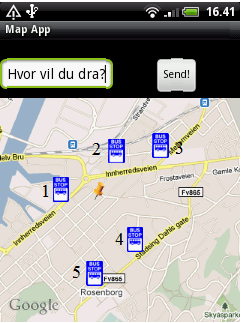
\includegraphics[scale=1]{TestingTheApplication/screen1.png}
  \end{center}
  \caption{Bus stop icons}
\label{fig:icons}
\end{wrapfigure}

Raaum's application uses an XML-file containing: bus stop locations, bus stop names and bus stop IDs, which does not contain sufficient information: information for several bus stops are missing. Also, the list also only contains one bus stop description per ''bus stop group''. A bus stop group consists of one or more bus stops with the same bus stop name. This is a problem in the extraction of real-time data, as a unique bus stop ID is necessary for each bus stop in a bus stop group. Figure \ref{fig:icons} illustrates this problem: only one icon is displayed for each stop group. 

Raaum's application has two sorting errors: one when the total travel time is equal for more than one route suggestion returned by BusTUC, and one when the distances are equal to two or more bus stops from the user's location. The error source is the use of HashMaps\footnote{http://docs.oracle.com/javase/1.4.2/docs/api/java/util/HashMap.html}, with total times or distances from the user's location to bus stops as keys. Keys in HashMaps are unique, because multiple equal keys overwrite the previous mapped value. In the total travel time issue, this leads to an exception as one or more route suggestions are overridden. In the distance issue,the error leads to a wrong display of bus stop icons on the map.

Raaum's application occasionally crashes during parsing of real-time data. This happens because the wrong node is extracted for some numbers. The extracted route numbers sometimes contain the letter ''N'', which in turn causes an exception when parsed as an integer. 

Queries with the new BusTUC syntax were meant to incorporate walking time to a bus stop in minutes. After testing, this was discovered to be ignored in BusTUC's reasoning. Time offsets may assure that unrealistic route suggestions are dropped. But on the other hand, real-time data is only available for bus departures in the ''near future'', and later real-time departure times are equal to the scheduled time. Syntacticly, it is a challenge to add text in the nested query syntax. A working syntax was: \emph{(Samfundet +2) fra Samfundet til Tiller etter $n$}. This was reasoned by BusTUC as if we wanted a bus departure after $n$.
 

Another issue is the handling of transfers, where two or more bus travels are needed to reach a destination. Raaum's application often suggests routes where the transfer bus departs before the first bus has arrived. This happens when the real-time data replaces the scheduled departure times returned from BusTUC, and no further sanity checks are performed. Although this does not cause an exception, the returned answers are unintelligent. 

The application crashes every time \emph{Lade} or \emph{Ranheim} is entered as input, while \emph{Lademoen} and \emph{Ranheim Stasjon} works. Testing with the BusTUC web-end and standard BusTUC syntax, works for all four. When the standard BusTUC syntax is used, BusTUC provides the correct bus stops. For Lade, this results in \emph{Lade all\'e}. No reasoning happens when using the new BusTUC syntax, except when a transfer is involved. BusTUC then maps the location to the bus stop correctly. Two examples are the queries: \emph{(Gl\o shaugen nord +2) til Lade}, and \emph{(Torget +2) til Lade}. The first query is successful, as a transfer is necessary to get to Lade. The second query leads to an  exception.

The list below summarises the errors and exceptions found and corrected during testing and debugging. There was no handling of these exceptions in Raaum's source code, but it was important for our future versions to introduce the necessary exception handling.
\begin{itemize}
\item{No handling of wrong or empty input}
\item{No handling of busy server}
\item{No handling of empty query results }
\item{Insufficient bus stop information}
\item{Wrong sorting of route suggestions}
\item{Wrong handling of routes involving transfers}
\item{Wrong parsing of real-time data}
\item{Wrong display of a user's location}
\item{ No handling of missing internet location}
\end{itemize}



\subsubsection{Adjustments Made to Raaum's Application}
It was necessary to modularise the existing source code because Raaum's code structure relied on to many dependencies, making any modifications difficult. Exception handling has also been addressed, for future development and for user testing. When Raaum's application was tested on Android devices(unplugged from a development machine), no detailed exception description was provided to the user. The only feedback was: ''The application has closed unexpectedly''. This needed to be improved because the average user is not capable of accessing exception descriptions through a debugger.

The HashMap issues were solved by re-implementing the sorting algorithms, and choosing a more object-oriented solution. HashMaps are fast when performing look-ups, but their usage did not fit this project. An object-oriented solution also aided the separation of code into multiple classes and activities. 

The HTML answers returned by BusTUC contained both JSON objects and text. The text answers were not used by Raaum's application, and should not be a part of the result returned from BusTUC. This is a BusTUC related issue, and not within TABuss' scope.

The transfer time issues were fixed by adding a validation after a route suggestion was received. The solution was simply to calculate the user's arrival time at the second bus stop, and compare with the real-time departure time.
\medskip
\begin{lstlisting}[caption={Real-time query result handling with logical soundness checks}, label=transferalgorithm]
depTime1 = Departure time from the first bus stop
depTime2 = Departure time from the second bus stop
walkingTime = Estimated two minutes of walking time
travelTime = Travel time from the first bus stop, to the second bus stop 
if (depTime1 + travelTime + walkingTime < depTime2)
	discard suggestion, and calculate a new route with updated arrival time at the second stop

 return suggestion
\end{lstlisting}
An example BusTUC query for a new route, is: \emph{(Sentrum+2) fra Sentrum til Ilsvika etter 1900)}.

\subsubsection{Testing BusTUC and The Real-time System}
The numbering scheme for bus stop IDs causes some problems: if there are two or more stops in a group, they can be separated by the fourth last digit in their IDs. This digit identifies whether passing buses are headed towards or away from the city centre. If there are two stops, buses heading towards the city centre pass the bus stop with 1 as the fourth last digit of its bus stop ID. Buses heading away from the city centre then pass the bus stop with 0 as the fourth last digit of its bus stop ID. An example is the stop group at \emph{Ila}:
\begin{itemize}
\item{Buses heading towards the city centre: 16011192}
\item{Buses heading away from the city centre: 16010192}
\end{itemize}

Problems occur for stop groups which only have one stop. Rune Andersen\footnote{http://www.ntnu.no/ansatte/rune.andersen}received emails from AtB, where it was explained that stop groups with one stop were assigned a bus stop ID with 0 as the fourth last digit. If we use \emph{Gudes gate} as an example, figure \ref{fig:gudes} implies that passing buses are headed away from the city centre(''fra byen''). However, a look-up in with AtB's route schedules shows that all buses pass Gudes Gate on a route heading towards the city centre.  A BusTUC query from \emph{sentrum} to Gudes gate suggests a route from sentrum to the end stop \emph{Asbj\o rnsens gate}, and then down to Gudes gate. Instead, the user could get off the bus on its way to the end stop, and walk(100 m) to Gudes gate. 

Another problem with BusTUC appears for queries with route 63. Then, the same bus stop ID is returned regardless of the direction of the passing buses. The tested queries were: \emph{Ila} to \emph{Dragvoll} and Ila to \emph{Ilsvika}. Ila to \emph{Buenget}, which is in the same direction as Ilsvika, returned the correct ID, as route 5 was returned instead of 63. Clearly, there are some inconsistencies, which seem to only affect certain stops and routes, but which can become problems when implementing new functionality. The project's supervisor(Rune) thought this occured as certain routes are ''circle'' routes, where buses only ever pass one stop in a stop group. However, for route 63, buses pass more than one of the stops in several of the stop groups. Still, only one bus stop ID is stored in BusTUC's knowledge base. This problem further affects Raaum's application's real-time updates of the departure times. Route suggestions are possibly updated with real-time departure times for buses travelling in the wrong direction: the two queries: \emph{(H\o gskoleringen +2) til Ilsvika} and \emph{(H\o gskoleringen +2) til Asbj\o rnsens gate}, return the same bus stop ID for route 63. Updating with real-time data returns equal departure times.

\vspace{10pt}
\begin{figure}[h]
  \begin{center}
    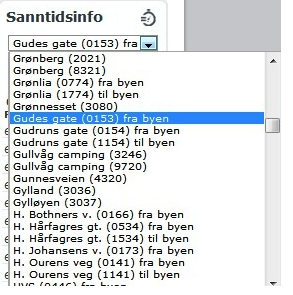
\includegraphics[scale=0.90]{TestingTheApplication/atb2.png}
  \end{center}
\label{fig:gudes}
  \caption{From atb.no: Gudes gate, with wrong direction given}
\label{fig:gudes}
  \end{figure}



